\begin{figure}[!htb]
    \begin{center}
    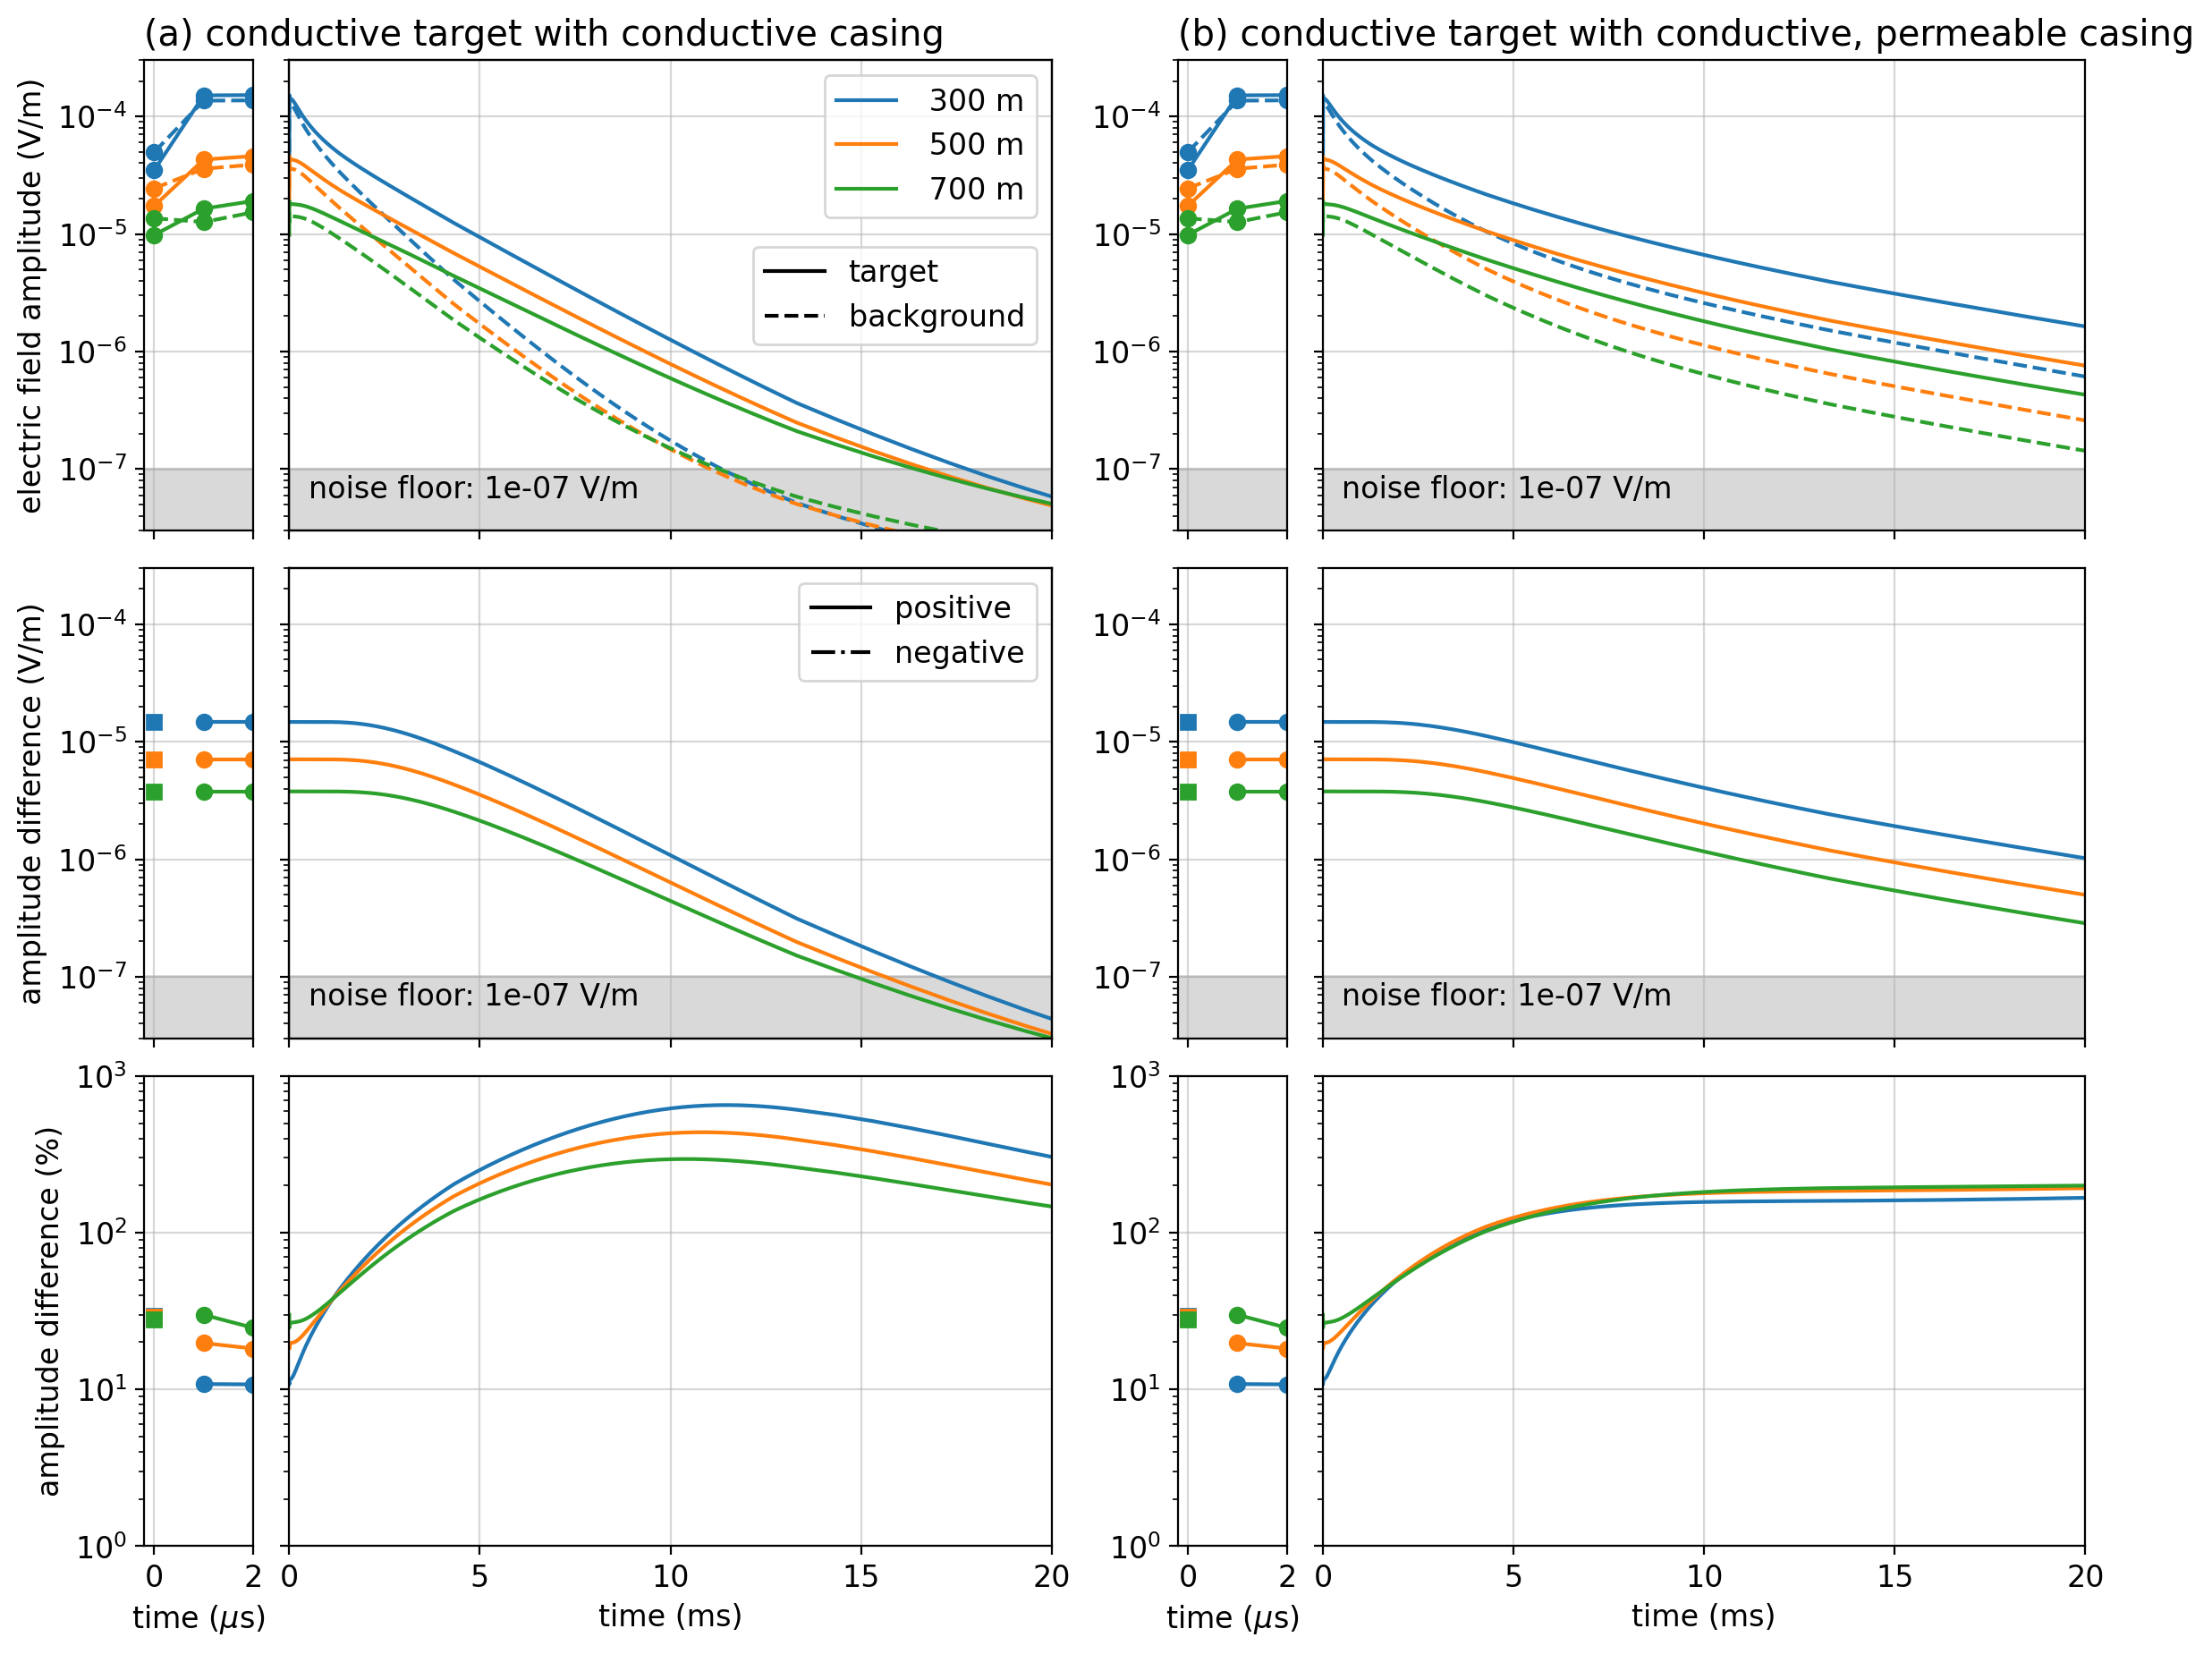
\includegraphics[width=0.9\textwidth]{figures/impact-of-wells-em-data.png}
    \end{center}
\caption{
    Amplitude of radial electric field data in a time-domain EM experiment with a conductive target (10 $\Omega$ m) as shown in Figure \ref{fig:impact-of-wells}.
    The data are collected along a line perpendicular to the transmitter wire, and the color of each line indicates the distance from the well where the timeseries is collected.
    The panels on the left show (a) the simulation for a conductive well which has a magnetic permeability equal to that of free space ($\mu_0$) and on the right, (b) we consider a well that has a permeability of $100 \mu_0$.
    The top plots show the simulated data for the scenario with (solid) and without (dashed) the conductive target. The thin plots on the left zoom in to the earliest times to show the DC response.
    The center plots show the difference between with and without the target. For the earliest times, a circle is used to denote where the amplitude difference is positive (the amplitude with the target is larger than without), and squares are used to show when the difference is negative. The bottom show that difference as a percentage of the results without the target.
}
\label{fig:impact-of-wells-em-data}
\end{figure}
